\documentclass[tikz,border=2mm]{standalone}
\usepackage{helvet}
\renewcommand{\familydefault}{\sfdefault}
\usetikzlibrary{arrows.meta,positioning}
\definecolor{datablue}{HTML}{4477AA}
\definecolor{methodteal}{HTML}{228833}
\definecolor{modelorange}{HTML}{CC6677}
\definecolor{impactpurple}{HTML}{AA3377}
\begin{document}
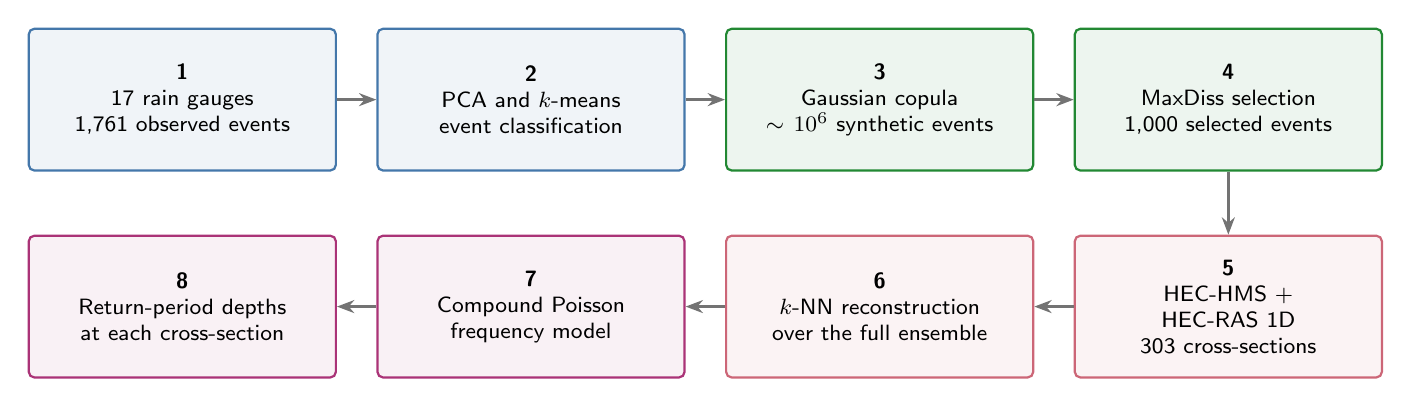
\begin{tikzpicture}[
  font=\fontsize{8}{9.4}\selectfont,
  stagebox/.style={rounded corners=2pt, line width=0.8pt, align=center,
    minimum width=39mm, minimum height=18mm, text width=34mm, inner sep=2mm},
  arrow/.style={-{Stealth[length=2.2mm]}, line width=0.9pt, draw=black!55}
]
\node[stagebox, draw=datablue, fill=datablue!8] (s1)
  {{\bfseries 1}\\17 rain gauges\\1,761 observed events};
\node[stagebox, draw=datablue, fill=datablue!8, right=5mm of s1] (s2)
  {{\bfseries 2}\\PCA and \(k\)-means\\event classification};
\node[stagebox, draw=methodteal, fill=methodteal!8, right=5mm of s2] (s3)
  {{\bfseries 3}\\Gaussian copula\\\(\sim 10^6\) synthetic events};
\node[stagebox, draw=methodteal, fill=methodteal!8, right=5mm of s3] (s4)
  {{\bfseries 4}\\MaxDiss selection\\1,000 selected events};

\node[stagebox, draw=impactpurple, fill=impactpurple!7, below=8mm of s1] (s8)
  {{\bfseries 8}\\Return-period depths\\at each cross-section};
\node[stagebox, draw=impactpurple, fill=impactpurple!7, below=8mm of s2] (s7)
  {{\bfseries 7}\\Compound Poisson\\frequency model};
\node[stagebox, draw=modelorange, fill=modelorange!8, below=8mm of s3] (s6)
  {{\bfseries 6}\\\(k\)-NN reconstruction\\over the full ensemble};
\node[stagebox, draw=modelorange, fill=modelorange!8, below=8mm of s4] (s5)
  {{\bfseries 5}\\HEC-HMS + HEC-RAS 1D\\303 cross-sections};

\draw[arrow] (s1) -- (s2);
\draw[arrow] (s2) -- (s3);
\draw[arrow] (s3) -- (s4);
\draw[arrow] (s4) -- (s5);
\draw[arrow] (s5) -- (s6);
\draw[arrow] (s6) -- (s7);
\draw[arrow] (s7) -- (s8);
\end{tikzpicture}
\end{document}
